\documentclass[12pt, letterpaper]{article}
%\documentclass[12pt, letterpaper]{amsart}

%%%%%%%%%%%% LANGUAGE & ENCODING %%%%%%%%%%%%%%%%%
\usepackage[english]{babel}
\usepackage[utf8]{inputenc}%%%% to process umlauts and accents directly
%\usepackage{indentfirst}
%\usepackage{ucs}

%%%%%%%%%%% PACKAGES %%%%%%%%%%%%%%%%%%%%%%%%%%%%%
% For Hyperlinks
\usepackage[colorlinks,linkcolor=cyan,citecolor=magenta]{hyperref}

% Common math packages
\usepackage{amsthm, amsmath, amsfonts, amssymb, esint, mathrsfs, mathtools}
\usepackage{tensor} % To handle multi-index notation
\usepackage[capitalize,nameinlink]{cleveref} % Nice references
\crefname{equation}{}{} % Removes Eq. from equation references
\numberwithin{equation}{section} % Number equations within each section separately

% Extra symbols
\usepackage{stmaryrd} % contains \owedge  for Kulkarni-Nomizu product and some other special characters
\usepackage{commath} % contains \norm \abs

% Some useful packages
\usepackage{verbatim} %%% enables \begin{comment}    \end{comment}
\usepackage{enumerate} % allows different types of indices
\usepackage{float} % Handling figures

%%%%%%%%%%% MARGINS %%%%%%%%%%%%%%%%%%%%%%%%%%%%%%%%
% Margins
\usepackage[top=1in, bottom=1in, left=1in, right=1in]{geometry}

%%%%%%%%%%% CUSTOM NOTATION  %%%%%%%%%%%%%%%%%%%%%%
\newcommand{\N}{\mathbb{N}}
\newcommand{\Z}{\mathbb{Z}}
\newcommand{\Q}{\mathbb{Q}}
\newcommand{\R}{\mathbb{R}}
\newcommand{\C}{\mathbb{C}}
\newcommand{\K}{\mathbb{K}}

\newcommand{\f}{\mathfrak}
\newcommand{\ul}{\underline}
\newcommand{\mb}{\mathbb}
\newcommand{\mr}{\mathrm}
\newcommand{\mf}{\mathbf}
\newcommand{\mc}{\mathcal}
\newcommand{\e}{\emph}
\newcommand{\vp}{\varphi}
\newcommand{\ve}{\varepsilon}

\newcommand{\vol}{\operatorname{Vol}}
\newcommand{\diam}{\operatorname{diam}}
\newcommand{\dist}{\operatorname{dist}}
\newcommand{\dv}{\operatorname{div}}
\newcommand{\tr}{\operatorname{tr}}

\newcommand{\dd}{\; \mathrm{d}} %%%% d for integration dx
\newcommand{\wt}{\widetilde}
\newcommand{\ol}{\overline}

%%%%%%%%%%% THEOREMS %%%%%%%%%%%%%%%%%%%%%%%%
\newtheorem{theorem}{Theorem}[section]
\newtheorem{lemma}[theorem]{Lemma}
\newtheorem{proposition}[theorem]{Proposition}
\newtheorem{conjecture}[theorem]{Conjecture}
\newtheorem{corollary}[theorem]{Corollary}
\newtheorem{claim}[theorem]{Claim}
\newtheorem{problem}[theorem]{Problem}
\newtheorem{remark}[theorem]{Remark}

\theoremstyle{definition}
\newtheorem{definition}[theorem]{Definition}

\theoremstyle{remark}
\newtheorem{example}[theorem]{Example}


%%%%%%%%%%% TITLE %%%%%%%%%%%%%%%%%%%
%\title[CIS625: Computational Learning Theory]{Computational Learning Theory Lecture Notes}
%\author[Notes by Martin Citoler-Saumell]{Martin Citoler-Saumell}
%\date{Spring 2017}
%\address{University of Pennsylvania\\ Philadelphia, PA 19104}
%\email{\href{mailto:martinci@math.upenn.edu}{martinci@math.upenn.edu}}

\title{Computational Learning Theory Lecture Notes}
\author{Martin Citoler-Saumell}
\date{CIS625 Spring 2017}

%%%%%%%%%%% DOCUMENT BEGINS %%%%%%%%%%%%
\begin{document}

%------------------------------------------------------------
%          LECTURE 8
%------------------------------------------------------------
\section{Lecture 8: 2017.03.20: Boosting}
Recall the PAC-learning scheme:
\begin{figure}[H]
\centering
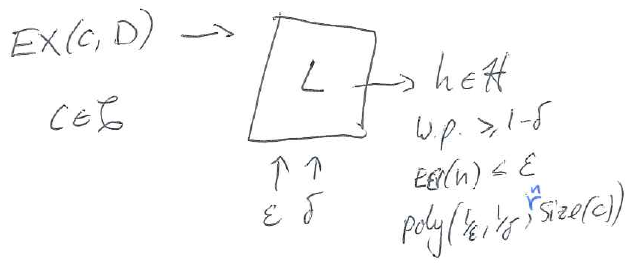
\includegraphics[width=0.6\linewidth]{img/pac-learning.png}
\caption{Scheme for PAC learning.}
\end{figure}


\subsubsection*{Hypothesis/Accuracy Boosting question:}
If we have an algorithm for PAC-learning some class $\mc C$ but only for \ul{fixed} $\ve_0$, does this imply a \ul{full} PAC algorithm (i.e. $\ve\to 0$)
\begin{remark}
Today we see that the answer to this question is Yes. By the remark above, this implies that the proof must use the fact that we are allowing \emph{any} distribution.
\end{remark}

\subsubsection{Confidence Boosting}
\begin{itemize}
\item Given algorithm $L$ that can achieve error $\ve$ ($\ve\to0$), but only for some \emph{fixed} value of $\delta=\delta_0$ (e.g. $\delta_0=\frac9{10}$) w.p. $1 - \frac9{10} = \frac1{10}$
\item Run $L$ k times, we get k hypothesis $h_1,\ldots,h_k$, which are independent. Note that each hypothesis has a chance $\frac1{10}$ of having error less than $\ve_0$ so if k is big enough, choosing the one with the best error has as high probability as we want to achieve error less than $\ve_0$. (It is basically the minimum of k independent Bernoulli trials).
\begin{align}
\mb P_{S_1,\ldots, S_k\sim D}\left[\forall 1\leq i \leq k, \quad Err(h_i)>\ve\right]\leq \delta_0^k,
\end{align}
which is less than any chosen $\delta$ if k is big enough. It is enough to pick $k\geq \frac{\log\left(\frac1\delta\right)}{\log\left(\frac1{\delta_0}\right)}$
\end{itemize}

\subsubsection{Accuracy Boosting}
Given algorithm $L$ such that for any distribution, w.p $\geq 1-\delta$, outputs h such that $Err(h) \leq \ve_0 = \frac12 - \gamma$ (i.e. slightly better than random guessing) (weak learning algorithm). One my try a similar thing as above but with taking a majority vote:
\begin{figure}[H]
\centering
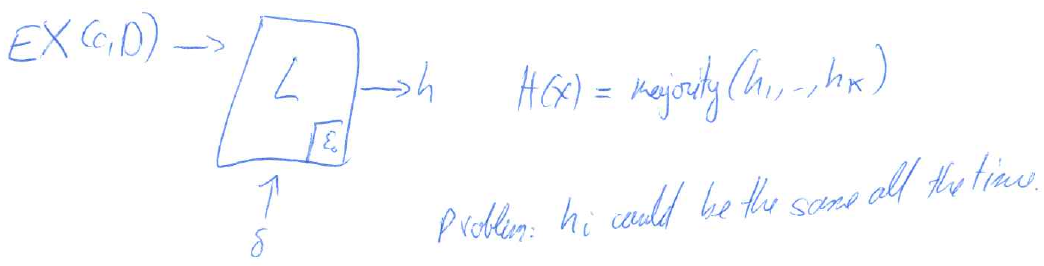
\includegraphics[width=0.6\linewidth]{img/majority.png}
\caption{Majority vote.}
\end{figure}
The problem is that $L$ could be evil and always output the same hypothesis. The key idea is to create filtered distributions to force $L$ to learn something ``new''.

\subsection{``Original'' Boosting construction (Schapire)}
\begin{enumerate}
\item Call weak learning algorithm L on $D_1 = D$ and we get $h_1$ such that $Err_{D_1}(h_1)\leq \ve_0$
\item We create a new distribution, $D_2$. To sample from $D_2$:
\begin{itemize}
\item Flip a fair coin.
\item If heads, sample $x\sim D_1$ until $h_1(x)\ne c(x)$.
\item If tails, sample until $h_1(x) = c(x)$. 
\end{itemize}
\begin{remark}
Note that if these conditions are not met for a lot of samples, then either $h_1$ or $\lnot h_1$ are already good enough hypothesis. This guarantees that $L$ cannot output $h_1$ or its negation as hypothesis because they would have error 50/50.
\end{remark}
Algebraically, this corresponds to modifying the weights of the original distribution, see the picture below.
\begin{figure}[H]
\centering
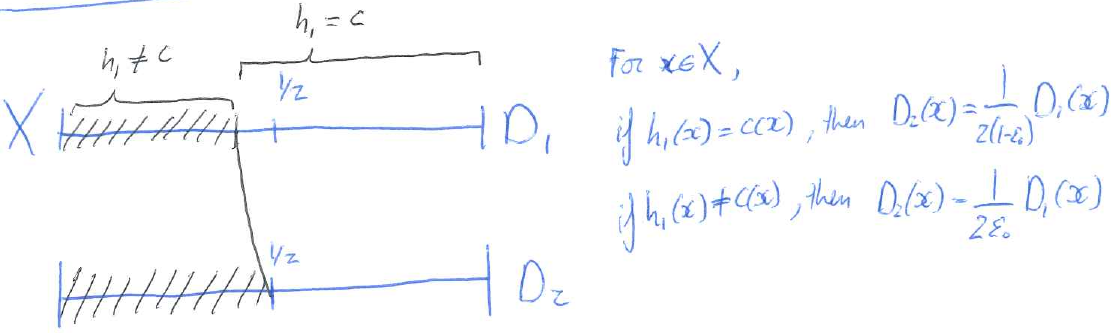
\includegraphics[width=0.6\linewidth]{img/weights.png}
\caption{Modify weights of original distribution.}
\end{figure}
Then we run $L$ on $EX(c,D_2)$ to get some $h_2\ne h_1$ such that $Err_{D_2}(h_2)\leq \ve_0$.
\item Define a distribution $D_3$. To sample from $D_3$:
\begin{itemize}
\item Draw $x\sim D_1$ until $h_1(x) \ne h_2(x)$. We will quickly get such a an $x$ by construction.
\item Create labeled example $\langle x, c(x) \rangle$.
\end{itemize}
Run $L$ on $EX(c, D_3)$ to get $h_3$ such that $Err_{D_3}(h_3)\leq \ve_0$.
\item Final hypothesis, for any $x$, $h(x) = \mathrm{majority}\lbrace h_1(x), h_2(x), h_3(x)\rbrace$.
\end{enumerate}
\begin{lemma}
$Err_{D_1}(h) \leq 3\ve_0^2 - 2\ve_0^3$.
\begin{remark}
\begin{figure}[H]
\centering
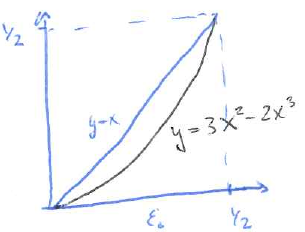
\includegraphics[width=0.3\linewidth]{img/boosting-bound.png}
\caption{$3x^2 - 2x^3$.}
\end{figure}
Note that it is a convex function below the line $\lbrace y = x\rbrace$. So we gain a little bit by boosting. Then we can iterate to obtain an arbitrary boosting.
\begin{figure}[H]
\centering
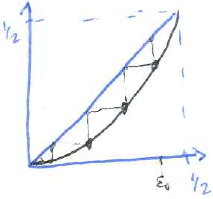
\includegraphics[width=0.3\linewidth]{img/boosting-iteration.png}
\caption{Boosting iterations.}
\end{figure}
Also note that the number of iterations needed to obtain error $\leq \ve$ is $\sim \log\log\frac1\ve$.
\end{remark}
\end{lemma}

We are actually changing the hypothesis space in the final algorithm. We output a ternary tree of majority hypotheses
\begin{figure}[H]
\centering
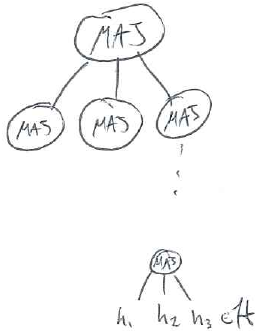
\includegraphics[width=0.3\linewidth]{img/majority-tree.png}
\caption{Majority tree.}
\end{figure}

\subsection{Adaboost (Freund/Schapire)}
\begin{itemize}
\item View input $S = (x_1, y_1), (x_2, y_2), \ldots, (x_m, y_m) \sim EX(c,D)$. Assume that $y_i\in\lbrace-1,1\rbrace$. We want to use the weak learning algorithm to find a hypothesis that is consistent with $S$, recall that as we saw before this is enough for PAC learning.
\item Start with $D_1$ the uniform distribution on $S$. If we can get $h$ such that $Err_{D_1}(h)<\frac1m$, then $h$ is consistent with $S$ and apply $VC$-theory.
\item Let's look at the ``code'', recall that the distributions refer to $S$.
\begin{enumerate}[]
\item $D_1 = \textrm{Unif}(S)$
\item for t in range $1,\ldots, T$
    \begin{enumerate}[-]
    \item run weak learning algorithm $L$ using $D_t$ to get some $h_t in \mc H$
    \item choose a weight $\alpha_t >= 0$ for the hypothesis $h_t$ (See analysis below)
    \item define the next distribution $D_{t+1}$
        \begin{align}D_{t+1}(x_i, y_i) = D_t(x_i, y_i)e^{-\alpha_ty_ih_t(x_i)}{Z_t},\end{align}
        where $Z_t$ is the normalization factor.
        \begin{remark}
        Note that $y_ih_t(x_i)$ is 1 if they agree or -1 otherwise. This means that we are increasing the weight on the places where $h_t$ was  wrong and reducing the weight on the ones where it was right.
        \end{remark}
    \end{enumerate}
\item Final classifier: $h(x) = sign(\sum_{t=1}^T\alpha_th_t(x))$
\end{enumerate}
\end{itemize}

\subsection*{Analysis}
\begin{remark}[Notation]
Let $\ve_i \coloneqq \mb P_{i\sim D_t}[h_t(x_i)\ne y_i]$ and $\gamma_t \coloneqq \frac12 -\ve_t$ ``advantage'' of $h_t$ over random guessing.
\end{remark}
If $y_i\ne H(x_i) = sign\left(\sum_{t=1}^T\alpha_th_t(x_i)\right)$, then $y_i\sum_{t=1}^T\alpha_th_t(x_i) \leq 0$, which implies that $e^{-\sum_{t=1}^T\alpha_th_t(x_i)}\geq 1$. So
\begin{align}\label{star}
\frac1m\abs{\lbrace i : H(x_i) \ne y_i \rbrace} \leq \frac1m \sum_ie^{-\sum_t\alpha_th_t(x_i)}.
\end{align}
Take any \ul{fixed} $i$, we can measure how much the distribution changes from $t$ to $t+1$
\begin{align}
 Z_t = \frac{D_t(x_i, y_i)e^{-\alpha_ty_ih_t(x_i))}}{D_{t+1}(x_i, y_i)}
\end{align}
Now we want take a look at how much the distribution has changed over $t$
\begin{align}
\prod_{t}^T Z_t = \frac{D_1(x_i, y_i)}{D_{T+1}(x_i, y_i)} e^{-y_i\sum_t\alpha_th_t(x_i)} = e^{-y_i\sum_t\alpha_th_t(x_i)},
\end{align}
since the $Z_t$'s are independent of $i$ so must be the right-hand-side above. We obtain,
\begin{align}
\prod_{t}^T Z_t = \frac mm \prod_{t}^T Z_t = \frac1 m \sum_i e^{-y_i\sum_t\alpha_th_t(x_i)},
\end{align}
so to estimate the error we only need to analyze the $Z_t$'s and recall that we are still free to choose the weights $\alpha_t$'s
\begin{align}
Z_t = \sum_i D_t(x_i, y_i)e^{-\alpha_ty_ih_t(x_i)},
\end{align}
therefore, we can choose $\alpha_t = \frac12 \ln\left(\frac{1-\ve_t}{\ve_t}\right)$ to obtain
\begin{align}
Z_t = (1-\ve_t)e^{-\alpha_t} + \ve_te^{\alpha_t} = \cdots \leq 2\sqrt{\ve_t(1-\ve_t)}.
\end{align}
Thus, we can bound the training error
\begin{align}
\textrm{training error} \leq \prod_t2\sqrt{\ve_t(1-\ve_t)} = \prod_t2\sqrt{1 - 4\gamma_t^2} \leq e^{-2\sum_t\gamma_t}.
\end{align}
We have arrived at the following result.
\begin{theorem}
Our training error on the original $S$ is bounded above by  $e^{-2\sum_t\gamma_t}$.
\end{theorem}

\end{document}
